%%%%%%%%%%%%%%%%%%%%%%%%%%%%%%%%%%%%%%%%%%%%%%%%%%%%%%%%%%%%%%%%%%% 
%                                                                 %
%                            CHAPTER                              %
%                                                                 %
%%%%%%%%%%%%%%%%%%%%%%%%%%%%%%%%%%%%%%%%%%%%%%%%%%%%%%%%%%%%%%%%%%% 

\chapter{Methods for genetic sequence alignment}
\label{ch:algoverzicht}


\section{Genetic sequence aligning}

The human genome (e.g. $HG19$) is used as a reference genome for all sequenced human DNA. However, The genetic code of all humans is slightly different. Genetic sequence alignment is the science where you try to align 2 sequences with each other so that the amount of differences is minimal. In this chapter, the most frequently used algorithms are examined.

\subsection{Alignment in general}

In genetic codes, there are 3 types of differences between the given sequence and the reference:

\begin{itemize}
	\item Insertion: one or more bases have been added in the genetic code in a specific spot.
	\item Deletion: one or more bases have been removed from the genetic code in a specific spot.
	\item Substitution: one or more bases have been substituted by other bases.
\end{itemize}

Inserts and deletions are often described by a single term, \emph{indel}. In literature, this is most often represented with a '$-$' character.\\

For example: if we want to align the following sequences:
\begin{lcverbatim}
	Seq1: ATATCGGC
	Seq2: ATCG
\end{lcverbatim}
The alignment itself can now be done in different ways. Possible alignments are:
\begin{lcverbatim}
	Alignment 1
	Seq1: AtaTCgGc
	Seq2: A--TC-G-
	Alignment 2
	Seq1: atATCGgc
	Seq2: --ATCG--
\end{lcverbatim}
Which alignment that is the actual output, depends on the algorithm and the given parameters.\\

Keep in mind, there is no one "correct" alignment. The core of the alignment algorithms is the same each time, but the parameters of these algorithms are changed depending on the application.

\section{Local VS global alignment}

To explain the difference between local and global alignment, we can take a look at the following example:

\begin{lcverbatim}
	The 2 DNA sequences:
	Seq1: TCCCAGTTTGTGTCAGGGGACACGAG
	Seq2: CGCCTCGTTTTCAGCAGTTATGTGCAGATC
	
	Alignment 1 :
	Seq1: -----------tccCAGTT-TGTGTCAGgggacacgag
	Seq2: cgcctcgttttcagCAGTTATGTG-CAGatc-------
	
	Alignment 2 :
	Seq1 : tcCCa-GTTTgt-GtCAGggg-acaC-GA-g
	Seq2 : cgCCtcGTTTtcaG-CAGttatgtgCaGAtc
\end{lcverbatim}

Both alignments are valid but different. The first alignment is \emph{locally aligned}. This means that the similarities are prioritized in the same region, with the similarity as high as possible. On the other hand, the second alignment is \emph{globally aligned}. Here the similarities over the full length of the sequences are used for the alignment. 

In practice, the local alignment is used most often, since it can give you information of 2 sequences that do not have (approximately) the same length.

\section{Commonly used algorithms}

In this section, we will take a look at some algorithms that are used most often for genetic sequence alignment.


The algorithms that are used most often are categorized in 2 ways: 

\begin{itemize}
	\item local alignment VS global alignments
	\item dynamic algorithms VS heuristic algorithms: dynamic algorithms are exact but slow and computationally demanding, whereas heuristic algorithms are faster but are approximations and the best alignment is not guaranteed.
\end{itemize}

Hereunder is a schematic view of some algorithms that are used in practice:

\begin{table}[H]
	\begin{tabular}{lllll}
		\cline{1-3}
		\multicolumn{1}{|l|}{}                          & \multicolumn{1}{l|}{\textbf{Dynamic programming}} & \multicolumn{1}{l|}{\textbf{Heuristic programming}} &  &  \\ \cline{1-3}
		\multicolumn{1}{|l|}{\textbf{Local alignment}}  & \multicolumn{1}{c|}{Smith-waterman}               & \multicolumn{1}{c|}{FASTA, BLAST}                   &  &  \\ \cline{1-3}
		\multicolumn{1}{|l|}{\textbf{Global alignment}} & \multicolumn{1}{c|}{Needleman-Wunsch}             & \multicolumn{1}{c|}{X}                              &  &  \\ \cline{1-3}
		&                                                   &                                                     &  & 
	\end{tabular}
	\caption{Classification of genetic alignment algorithms}
\end{table}


Keep in mind, a lot of other claimed "algorithms" (for example BFAST, ...), are accelerated versions of the Smith-Waterman algorithm.

\subsection{Needleman-Wunsch}
Needleman and Wunch proposed a new algorithm for genetic sequence alignment in 1970, now known as the \emph{Needleman-Wunsch} (N-W) algorithm. Since this algorithm is meant for global alignment. Since global alignment is seldomly used in practice, further analysis of the algorithm will not be done. However, N-W has a lot of similarities with the Smith-Waterman algorithm, discussed in the next section.

\subsection{Smith-Waterman}
%explanation for SW
The \emph{Smith-Waterman} (S-W) algorithm was first proposed by Temple F. Smith and Michael S. Waterman in 1981. It is a variation on (N-W), adapted for local alignment. It is a dynamic programming technique, so the optimal local alignment is guaranteed. \\

The core of the algorithm is a matrix fillup, with data dependencies on the previous cells. Hereunder an analysis of the algorithm:

\begin{enumerate}
	\item Symbols used in the analysis:
	
	Let sequences $A = a_1 a_2 a_3 \dots a_n$ and $B = b_1 b_2 b_3 \dots b_m$ be the sequences that need to be locally aligned. Here $n$ and $m$ are the lengths of sequence $A$ and $B$
	
	\item Define the parameters: 
	
	\begin{itemize}
		\item Define $s(a,b)$ be the \emph{similarity matrix} (sometimes also called the \emph{substitution matrix}) for the two sequences. It is used for "rewarding" when $a_i = b_j$ and "punishing" when $a_i \neq b_j$.
		
		In the most general way, we define the similarity score as a matrix of values, e.g.:
		
		\begin{table}[H]
			\centering
			\begin{tabular}{|r|r|r|r|r|}
				\hline
				& \textbf{A} & \textbf{C} & \textbf{G} & \textbf{T} \\ \hline
				\textbf{A} & 3          & -3         & -3         & -3         \\ \hline
				\textbf{C} & -3         & 3          & -3         & -3         \\ \hline
				\textbf{G} & -3         & -3         & 3          & -3         \\ \hline
				\textbf{T} & -3         & -3         & -3         & 3          \\ \hline
			\end{tabular}
			
			\caption{\centering Similarity matrix example}
		\end{table}
		
		Often, there are only 2 scores used (equal or not equal). In this case, the similarity matrix can be condensed as follows:
		
		\begin{align*}
		s(a_i,b_j)=
		\begin{cases}
		+3, \quad a_i=b_j     \\
		-3, \quad a_i\neq b_j
		\end{cases}
		\end{align*}
		
		\item Define $d$ as the \emph{gap penalty} which regulates the score for an insertion or a deletion. This parameter can be:
		
		\begin{itemize}
			\item \emph{Linear}: The penalty is constant. So, in this case, it doesn't matter e.g. the previous was also a gap.
			\item \emph{Affine}: An affine gap penalty considers gap opening and extension separately. For the sake of simplicity, this analysis will not cover it. The algorithm can be extended to include this affine gap penalty, but this would make the algorithm more complex and we would limit our ability to develop possible accelerations.
		\end{itemize}
		
		
	\end{itemize}
	
	
	\item The initialization: We construct a scoring matrix $H$ with dimensions $(n+1)\times(m+1)$. The first column and first row we initialize with $0$.
	
	For example: if we want to align the sequences A = $TGTTACGG$ and B = $GGTTGACTA$:
	
	\begin{table}[H]
		\centering
		\begin{tabular}{rrrrrrrrrr}
			&                        & T                      & G                      & T                      & T                      & A                      & C                      & G                      & G                      \\ \cline{2-10} 
			\multicolumn{1}{r|}{}  & \multicolumn{1}{r|}{0} & \multicolumn{1}{r|}{0} & \multicolumn{1}{r|}{0} & \multicolumn{1}{r|}{0} & \multicolumn{1}{r|}{0} & \multicolumn{1}{r|}{0} & \multicolumn{1}{r|}{0} & \multicolumn{1}{r|}{0} & \multicolumn{1}{r|}{0} \\ \cline{2-10} 
			\multicolumn{1}{r|}{G} & \multicolumn{1}{r|}{0} & \multicolumn{1}{r|}{}  & \multicolumn{1}{r|}{}  & \multicolumn{1}{r|}{}  & \multicolumn{1}{r|}{}  & \multicolumn{1}{r|}{}  & \multicolumn{1}{r|}{}  & \multicolumn{1}{r|}{}  & \multicolumn{1}{r|}{}  \\ \cline{2-10} 
			\multicolumn{1}{r|}{G} & \multicolumn{1}{r|}{0} & \multicolumn{1}{r|}{}  & \multicolumn{1}{r|}{}  & \multicolumn{1}{r|}{}  & \multicolumn{1}{r|}{}  & \multicolumn{1}{r|}{}  & \multicolumn{1}{r|}{}  & \multicolumn{1}{r|}{}  & \multicolumn{1}{r|}{}  \\ \cline{2-10} 
			\multicolumn{1}{r|}{T} & \multicolumn{1}{r|}{0} & \multicolumn{1}{r|}{}  & \multicolumn{1}{r|}{}  & \multicolumn{1}{r|}{}  & \multicolumn{1}{r|}{}  & \multicolumn{1}{r|}{}  & \multicolumn{1}{r|}{}  & \multicolumn{1}{r|}{}  & \multicolumn{1}{r|}{}  \\ \cline{2-10} 
			\multicolumn{1}{r|}{T} & \multicolumn{1}{r|}{0} & \multicolumn{1}{r|}{}  & \multicolumn{1}{r|}{}  & \multicolumn{1}{r|}{}  & \multicolumn{1}{r|}{}  & \multicolumn{1}{r|}{}  & \multicolumn{1}{r|}{}  & \multicolumn{1}{r|}{}  & \multicolumn{1}{r|}{}  \\ \cline{2-10} 
			\multicolumn{1}{r|}{G} & \multicolumn{1}{r|}{0} & \multicolumn{1}{r|}{}  & \multicolumn{1}{r|}{}  & \multicolumn{1}{r|}{}  & \multicolumn{1}{r|}{}  & \multicolumn{1}{r|}{}  & \multicolumn{1}{r|}{}  & \multicolumn{1}{r|}{}  & \multicolumn{1}{r|}{}  \\ \cline{2-10} 
			\multicolumn{1}{r|}{A} & \multicolumn{1}{r|}{0} & \multicolumn{1}{r|}{}  & \multicolumn{1}{r|}{}  & \multicolumn{1}{r|}{}  & \multicolumn{1}{r|}{}  & \multicolumn{1}{r|}{}  & \multicolumn{1}{r|}{}  & \multicolumn{1}{r|}{}  & \multicolumn{1}{r|}{}  \\ \cline{2-10} 
			\multicolumn{1}{r|}{C} & \multicolumn{1}{r|}{0} & \multicolumn{1}{r|}{}  & \multicolumn{1}{r|}{}  & \multicolumn{1}{r|}{}  & \multicolumn{1}{r|}{}  & \multicolumn{1}{r|}{}  & \multicolumn{1}{r|}{}  & \multicolumn{1}{r|}{}  & \multicolumn{1}{r|}{}  \\ \cline{2-10} 
			\multicolumn{1}{r|}{T} & \multicolumn{1}{r|}{0} & \multicolumn{1}{r|}{}  & \multicolumn{1}{r|}{}  & \multicolumn{1}{r|}{}  & \multicolumn{1}{r|}{}  & \multicolumn{1}{r|}{}  & \multicolumn{1}{r|}{}  & \multicolumn{1}{r|}{}  & \multicolumn{1}{r|}{}  \\ \cline{2-10} 
			\multicolumn{1}{r|}{A} & \multicolumn{1}{r|}{0} & \multicolumn{1}{r|}{}  & \multicolumn{1}{r|}{}  & \multicolumn{1}{r|}{}  & \multicolumn{1}{r|}{}  & \multicolumn{1}{r|}{}  & \multicolumn{1}{r|}{}  & \multicolumn{1}{r|}{}  & \multicolumn{1}{r|}{}  \\ \cline{2-10} 
		\end{tabular}
		\caption{\centering Example of the initialization of the scoring matrix}
	\end{table}
	
	\item Matrix fill in:
	We fill in the matrix using the following formula:
	
	\begin{align*}
	H_{ij}= max
	\begin{cases}
	H_{i-1,j-1} + s(a_i, b_j),\\
	H_{i-1,j} - d,\\
	H_{i,j-1} - d,\\
	0
	\end{cases}
	\end{align*}
	
	If we keep in mind that the value of a cell may never be lower than 0, we can represent the data dependencies in the following schematic:
	
	
	\begin{figure}[H]
		\centering
		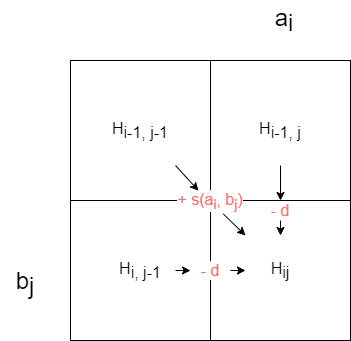
\includegraphics[width=0.5\textwidth]{ExisMethods/Dependencies_SW.png}
		\caption{Data dependencies in the $H$ matrix}
		\label{fig:DatDep}
	\end{figure}
	
	Where $s(a,b)$ and $d$ are the parameters of the algorithm. If we use the following values as an example:
	
	\begin{align*}
	s(a_i,b_j)=
	\begin{cases}
	+3, \quad a_i=b_j     \\
	-3, \quad a_i\neq b_j
	\end{cases} \qquad \text{and} \qquad d = 2
	\end{align*}
	
	We can now fill up the scoring matrix $H$:
	
	\begin{table}[H]
		\centering
		\begin{tabular}{rrrrrrrrrr}
			&                        & T                      & G                      & T                      & T                      & A                       & C                       & G                       & G                      \\ \cline{2-10} 
			\multicolumn{1}{r|}{}  & \multicolumn{1}{r|}{0} & \multicolumn{1}{r|}{0} & \multicolumn{1}{r|}{0} & \multicolumn{1}{r|}{0} & \multicolumn{1}{r|}{0} & \multicolumn{1}{r|}{0}  & \multicolumn{1}{r|}{0}  & \multicolumn{1}{r|}{0}  & \multicolumn{1}{r|}{0} \\ \cline{2-10} 
			\multicolumn{1}{r|}{G} & \multicolumn{1}{r|}{0} & \multicolumn{1}{r|}{0} & \multicolumn{1}{r|}{3} & \multicolumn{1}{r|}{1} & \multicolumn{1}{r|}{0} & \multicolumn{1}{r|}{0}  & \multicolumn{1}{r|}{0}  & \multicolumn{1}{r|}{3}  & \multicolumn{1}{r|}{3} \\ \cline{2-10} 
			\multicolumn{1}{r|}{G} & \multicolumn{1}{r|}{0} & \multicolumn{1}{r|}{0} & \multicolumn{1}{r|}{3} & \multicolumn{1}{r|}{1} & \multicolumn{1}{r|}{0} & \multicolumn{1}{r|}{0}  & \multicolumn{1}{r|}{0}  & \multicolumn{1}{r|}{3}  & \multicolumn{1}{r|}{6} \\ \cline{2-10} 
			\multicolumn{1}{r|}{T} & \multicolumn{1}{r|}{0} & \multicolumn{1}{r|}{3} & \multicolumn{1}{r|}{1} & \multicolumn{1}{r|}{6} & \multicolumn{1}{r|}{4} & \multicolumn{1}{r|}{2}  & \multicolumn{1}{r|}{0}  & \multicolumn{1}{r|}{1}  & \multicolumn{1}{r|}{4} \\ \cline{2-10} 
			\multicolumn{1}{r|}{T} & \multicolumn{1}{r|}{0} & \multicolumn{1}{r|}{3} & \multicolumn{1}{r|}{1} & \multicolumn{1}{r|}{4} & \multicolumn{1}{r|}{9} & \multicolumn{1}{r|}{7}  & \multicolumn{1}{r|}{5}  & \multicolumn{1}{r|}{3}  & \multicolumn{1}{r|}{2} \\ \cline{2-10} 
			\multicolumn{1}{r|}{G} & \multicolumn{1}{r|}{0} & \multicolumn{1}{r|}{1} & \multicolumn{1}{r|}{6} & \multicolumn{1}{r|}{4} & \multicolumn{1}{r|}{7} & \multicolumn{1}{r|}{6}  & \multicolumn{1}{r|}{4}  & \multicolumn{1}{r|}{8}  & \multicolumn{1}{r|}{6} \\ \cline{2-10} 
			\multicolumn{1}{r|}{A} & \multicolumn{1}{r|}{0} & \multicolumn{1}{r|}{0} & \multicolumn{1}{r|}{4} & \multicolumn{1}{r|}{3} & \multicolumn{1}{r|}{5} & \multicolumn{1}{r|}{10} & \multicolumn{1}{r|}{8}  & \multicolumn{1}{r|}{6}  & \multicolumn{1}{r|}{5} \\ \cline{2-10} 
			\multicolumn{1}{r|}{C} & \multicolumn{1}{r|}{0} & \multicolumn{1}{r|}{0} & \multicolumn{1}{r|}{2} & \multicolumn{1}{r|}{1} & \multicolumn{1}{r|}{3} & \multicolumn{1}{r|}{8}  & \multicolumn{1}{r|}{13} & \multicolumn{1}{r|}{11} & \multicolumn{1}{r|}{9} \\ \cline{2-10} 
			\multicolumn{1}{r|}{T} & \multicolumn{1}{r|}{0} & \multicolumn{1}{r|}{3} & \multicolumn{1}{r|}{1} & \multicolumn{1}{r|}{5} & \multicolumn{1}{r|}{4} & \multicolumn{1}{r|}{6}  & \multicolumn{1}{r|}{11} & \multicolumn{1}{r|}{10} & \multicolumn{1}{r|}{8} \\ \cline{2-10} 
			\multicolumn{1}{r|}{A} & \multicolumn{1}{r|}{0} & \multicolumn{1}{r|}{1} & \multicolumn{1}{r|}{0} & \multicolumn{1}{r|}{3} & \multicolumn{1}{r|}{2} & \multicolumn{1}{r|}{7}  & \multicolumn{1}{r|}{9}  & \multicolumn{1}{r|}{8}  & \multicolumn{1}{r|}{7} \\ \cline{2-10} 
		\end{tabular}
		\caption{\centering Example of a populated scoring matrix}
	\end{table}
	
	
	\item Traceback: We start at the cell with the highest score in the matrix $H$. Starting here we only move left, up or diagonally (left-up) to the cell on which the value in the cell was based until we hit a cell with value $0$.
	
	
	\begin{table}[H]
		\centering
		\begin{tabular}{rrrrrrrrrr}
			&                        & T                                              & G                                              & T                                              & T                                              & A                                               & C                                               & G                       & G                      \\ \cline{2-10} 
			\multicolumn{1}{r|}{}  & \multicolumn{1}{r|}{0} & \multicolumn{1}{r|}{0}                         & \multicolumn{1}{r|}{0}                         & \multicolumn{1}{r|}{0}                         & \multicolumn{1}{r|}{0}                         & \multicolumn{1}{r|}{0}                          & \multicolumn{1}{r|}{0}                          & \multicolumn{1}{r|}{0}  & \multicolumn{1}{r|}{0} \\ \cline{2-10} 
			\multicolumn{1}{r|}{G} & \multicolumn{1}{r|}{0} & \multicolumn{1}{r|}{\cellcolor[HTML]{FFCCC9}0} & \multicolumn{1}{r|}{3}                         & \multicolumn{1}{r|}{1}                         & \multicolumn{1}{r|}{0}                         & \multicolumn{1}{r|}{0}                          & \multicolumn{1}{r|}{0}                          & \multicolumn{1}{r|}{3}  & \multicolumn{1}{r|}{3} \\ \cline{2-10} 
			\multicolumn{1}{r|}{G} & \multicolumn{1}{r|}{0} & \multicolumn{1}{r|}{0}                         & \multicolumn{1}{r|}{\cellcolor[HTML]{DAE8FC}3} & \multicolumn{1}{r|}{1}                         & \multicolumn{1}{r|}{0}                         & \multicolumn{1}{r|}{0}                          & \multicolumn{1}{r|}{0}                          & \multicolumn{1}{r|}{3}  & \multicolumn{1}{r|}{6} \\ \cline{2-10} 
			\multicolumn{1}{r|}{T} & \multicolumn{1}{r|}{0} & \multicolumn{1}{r|}{3}                         & \multicolumn{1}{r|}{1}                         & \multicolumn{1}{r|}{\cellcolor[HTML]{DAE8FC}6} & \multicolumn{1}{r|}{4}                         & \multicolumn{1}{r|}{2}                          & \multicolumn{1}{r|}{0}                          & \multicolumn{1}{r|}{1}  & \multicolumn{1}{r|}{4} \\ \cline{2-10} 
			\multicolumn{1}{r|}{T} & \multicolumn{1}{r|}{0} & \multicolumn{1}{r|}{3}                         & \multicolumn{1}{r|}{1}                         & \multicolumn{1}{r|}{4}                         & \multicolumn{1}{r|}{\cellcolor[HTML]{DAE8FC}9} & \multicolumn{1}{r|}{7}                          & \multicolumn{1}{r|}{5}                          & \multicolumn{1}{r|}{3}  & \multicolumn{1}{r|}{2} \\ \cline{2-10} 
			\multicolumn{1}{r|}{G} & \multicolumn{1}{r|}{0} & \multicolumn{1}{r|}{1}                         & \multicolumn{1}{r|}{6}                         & \multicolumn{1}{r|}{4}                         & \multicolumn{1}{r|}{\cellcolor[HTML]{DAE8FC}7} & \multicolumn{1}{r|}{6}                          & \multicolumn{1}{r|}{4}                          & \multicolumn{1}{r|}{8}  & \multicolumn{1}{r|}{6} \\ \cline{2-10} 
			\multicolumn{1}{r|}{A} & \multicolumn{1}{r|}{0} & \multicolumn{1}{r|}{0}                         & \multicolumn{1}{r|}{4}                         & \multicolumn{1}{r|}{3}                         & \multicolumn{1}{r|}{5}                         & \multicolumn{1}{r|}{\cellcolor[HTML]{DAE8FC}10} & \multicolumn{1}{r|}{8}                          & \multicolumn{1}{r|}{6}  & \multicolumn{1}{r|}{5} \\ \cline{2-10} 
			\multicolumn{1}{r|}{C} & \multicolumn{1}{r|}{0} & \multicolumn{1}{r|}{0}                         & \multicolumn{1}{r|}{2}                         & \multicolumn{1}{r|}{1}                         & \multicolumn{1}{r|}{3}                         & \multicolumn{1}{r|}{8}                          & \multicolumn{1}{r|}{\cellcolor[HTML]{34CDF9}13} & \multicolumn{1}{r|}{11} & \multicolumn{1}{r|}{9} \\ \cline{2-10} 
			\multicolumn{1}{r|}{T} & \multicolumn{1}{r|}{0} & \multicolumn{1}{r|}{3}                         & \multicolumn{1}{r|}{1}                         & \multicolumn{1}{r|}{5}                         & \multicolumn{1}{r|}{4}                         & \multicolumn{1}{r|}{6}                          & \multicolumn{1}{r|}{11}                         & \multicolumn{1}{r|}{10} & \multicolumn{1}{r|}{8} \\ \cline{2-10} 
			\multicolumn{1}{r|}{A} & \multicolumn{1}{r|}{0} & \multicolumn{1}{r|}{1}                         & \multicolumn{1}{r|}{0}                         & \multicolumn{1}{r|}{3}                         & \multicolumn{1}{r|}{2}                         & \multicolumn{1}{r|}{7}                          & \multicolumn{1}{r|}{9}                          & \multicolumn{1}{r|}{8}  & \multicolumn{1}{r|}{7} \\ \cline{2-10} 
		\end{tabular}
		\caption{\centering Example of a traceback in S-W}
	\end{table}
	
	From this traceback we can now deduce the following alignment:
	
\begin{lcverbatim}
GTT-AC
||||||
GTTGAC
\end{lcverbatim}
	
	This alignment is the output of our algorithm.
	
\end{enumerate}

\section{Problem definition and algorithm selection}

\subsection{Mapping to a reference genome}

\subsection{Clinical application}